\begin{center}
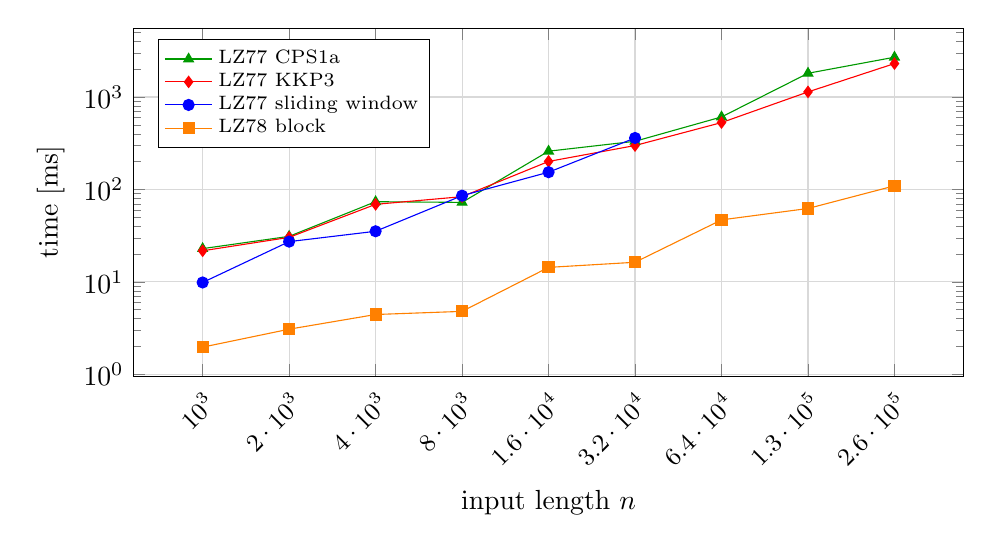
\begin{tikzpicture}
\begin{axis}[
  width = \linewidth, height = 6cm,
  xlabel = {input length $n$}, ylabel = {time [ms]},
  xmode = log, ymode = log,
  legend pos = north west, legend cell align = left,
  legend style = {font = \scriptsize, row sep = -2pt, inner sep = 2pt},
  xmajorgrids = true, ymajorgrids = true,
  xminorgrids = false, yminorgrids = false,
  minor tick num = 0,
  grid style = {draw = gray!30},
  xtick = {1000, 2000, 4000, 8000, 16000, 32000, 64000, 128000, 256000},
  xticklabels = {$10^{3}$, $2 \cdot 10^{3}$, $4 \cdot 10^{3}$, $8 \cdot 10^{3}$, $1.6 \cdot 10^{4}$, $3.2 \cdot 10^{4}$, $6.4 \cdot 10^{4}$, $1.3 \cdot 10^{5}$, $2.6 \cdot 10^{5}$},
  x tick label style = {rotate = 45, anchor = north east, font = \small},
]
\addplot[color = green!60!black, mark = triangle*] coordinates {(1000, 22.91) (2000, 31.1) (4000, 73.73) (8000, 72.49) (16000, 259.4) (32000, 331.96) (64000, 608.61) (128000, 1806.19) (256000, 2694.28)};
\addlegendentry{LZ77 CPS1a}
\addplot[color = red, mark = diamond*] coordinates {(1000, 21.71) (2000, 30.33) (4000, 69.04) (8000, 83.58) (16000, 200.89) (32000, 298.71) (64000, 528.87) (128000, 1135.06) (256000, 2299.99)};
\addlegendentry{LZ77 KKP3}
\addplot[color = blue, mark = *] coordinates {(1000, 9.86) (2000, 27.27) (4000, 35.3) (8000, 85.68) (16000, 153.7) (32000, 360.45)};
\addlegendentry{LZ77 sliding window}
\addplot[color = orange, mark = square*] coordinates {(1000, 1.97) (2000, 3.08) (4000, 4.44) (8000, 4.8) (16000, 14.36) (32000, 16.31) (64000, 46.87) (128000, 62.27) (256000, 109.43)};
\addlegendentry{LZ78 block}
\end{axis}
\end{tikzpicture}
\captionof{figure}{Fibonacci, encoding time.}
\label{fig:Fibonacci-encoding}
\end{center}

\begin{center}
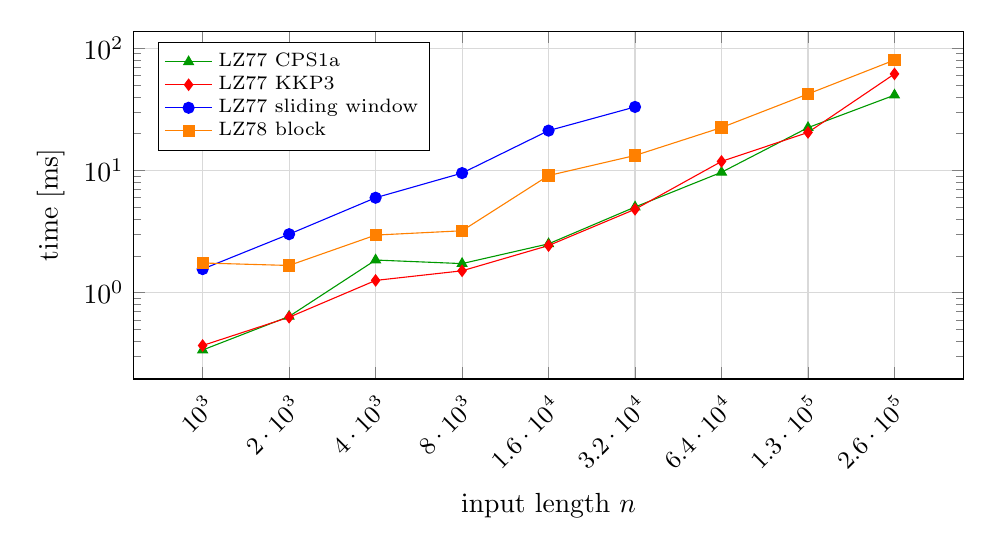
\begin{tikzpicture}
\begin{axis}[
  width = \linewidth, height = 6cm,
  xlabel = {input length $n$}, ylabel = {time [ms]},
  xmode = log, ymode = log,
  legend pos = north west, legend cell align = left,
  legend style = {font = \scriptsize, row sep = -2pt, inner sep = 2pt},
  xmajorgrids = true, ymajorgrids = true,
  xminorgrids = false, yminorgrids = false,
  minor tick num = 0,
  grid style = {draw = gray!30},
  xtick = {1000, 2000, 4000, 8000, 16000, 32000, 64000, 128000, 256000},
  xticklabels = {$10^{3}$, $2 \cdot 10^{3}$, $4 \cdot 10^{3}$, $8 \cdot 10^{3}$, $1.6 \cdot 10^{4}$, $3.2 \cdot 10^{4}$, $6.4 \cdot 10^{4}$, $1.3 \cdot 10^{5}$, $2.6 \cdot 10^{5}$},
  x tick label style = {rotate = 45, anchor = north east, font = \small},
]
\addplot[color = green!60!black, mark = triangle*] coordinates {(1000, 0.34) (2000, 0.64) (4000, 1.85) (8000, 1.73) (16000, 2.51) (32000, 5.02) (64000, 9.66) (128000, 22.39) (256000, 41.29)};
\addlegendentry{LZ77 CPS1a}
\addplot[color = red, mark = diamond*] coordinates {(1000, 0.37) (2000, 0.63) (4000, 1.26) (8000, 1.51) (16000, 2.43) (32000, 4.81) (64000, 11.85) (128000, 20.46) (256000, 61.55)};
\addlegendentry{LZ77 KKP3}
\addplot[color = blue, mark = *] coordinates {(1000, 1.56) (2000, 3.01) (4000, 5.98) (8000, 9.51) (16000, 21.16) (32000, 33.06)};
\addlegendentry{LZ77 sliding window}
\addplot[color = orange, mark = square*] coordinates {(1000, 1.75) (2000, 1.67) (4000, 2.96) (8000, 3.21) (16000, 9.08) (32000, 13.25) (64000, 22.42) (128000, 42.2) (256000, 79.93)};
\addlegendentry{LZ78 block}
\end{axis}
\end{tikzpicture}
\captionof{figure}{Fibonacci, decoding time.}
\label{fig:Fibonacci-decoding}
\end{center}

\begin{center}
\begin{tabular}{lrrrrrr}
\hline
algorithm & $n$ & $\alpha$ & $z$ & $\rho$ & encode [ms] & decode [ms] \\
\hline
LZ77 sliding window & 32000 & 2 & 22 & 0.0213 & 469.08 & 64.52 \\
LZ78 block & 32000 & 2 & 1050 & 0.3298 & 152.9 & 35.42 \\
LZ77 CPS1a & 32000 & 2 & 22 & 0.0206 & 605.42 & 8.11 \\
LZ77 KKP3 & 32000 & 2 & 22 & 0.0206 & 545.25 & 10.96 \\
\hline
\end{tabular}
\captionof{table}{Fibonacci: the Fibonacci word.}
\label{tab:Fibonacci}
\end{center}
